\section{Math}

The two types of springs used in AEM are normal springs and shear springs.

For the normal springs 

\begin{equation}
K_n = \frac{E d T}{a}
\label{eq:Normal_spring}
\end{equation}

and for the shear springs

\begin{equation}
K_s = \frac{G d T}{a}
\label{eq:Shear_spring}
\end{equation}

\begin{figure}[H]
\centering
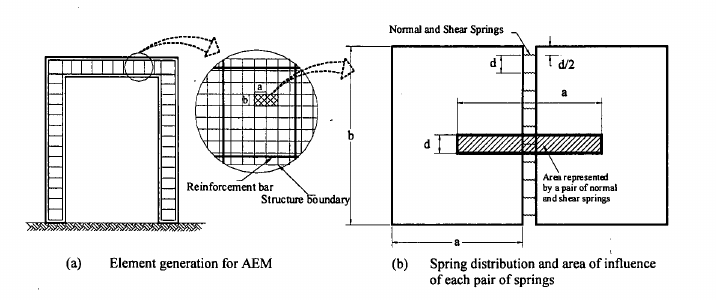
\includegraphics[width=0.6\textwidth]{../Modelling_anatomy.png}
\caption{Modelling of structure to AEM [\cite{First_AEM}]}
\label{fig:Modelling_anatomy}
\end{figure}

As can be seen in the figure the Applied Element Method makes use of springs to model the interactions between small elements.  The elements are assumed to be connected with pairs of normal and shear springs, these springs are located at contact locations which are distributed across the element edges. 
A pair of springs represent stresses and deformations of a certain area.  in Figure \ref{fig:Modelling_anatomy} this area is the darker hatched area.  Equations \ref{eq:Normal_spring} and \ref{eq:Shear_spring} show the spring stiffness for the pair of springs. $a$ is the length of the area represented by the spring, $d$ is both the distance between the springs and the height of the represented area. $E$ and $G$ are the Young's and Shear modulus of the material.  Finally $T$ is the thickness of the material. [\cite{First_AEM}]

The next section of mathematical breakdown of the method is extracted from [\cite{First_AEM}].  This paper was published as part of a series of papers explaining various ways to use the AEM method to model different situations.  These paper lists and the modelling methods using AEM is shown in Figure \ref{fig:AEM_paper_series} which is a table extracted from [\cite{First_AEM}].

\begin{figure}[H]
\centering
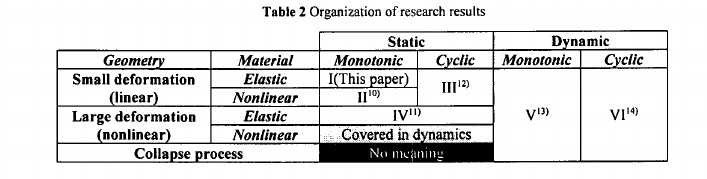
\includegraphics[width=0.6\textwidth]{../AEM_paper_series.png}
\caption{Breakdown of Papers published with modelling methods using AEM [\cite{First_AEM}]}
\label{fig:AEM_paper_series}
\end{figure}

\newpage

\subsection{Static Monotonic Small Deformations of Elastic Material}

\begin{figure}[H]
\centering
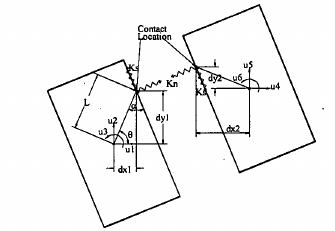
\includegraphics[width=0.45\textwidth]{../Element_shape_DOF.png}
\caption{Degrees of Freedom and Element shape with Contact location shown [\cite{First_AEM}]}
\label{fig:Element_shape_DOF}
\end{figure}


With the assumption of three degrees of freedom for each element namely displacement in the x and y direction and rotation in the x-y plane.  These degrees of freedom represent the rigid body motion of each element.  What should be noted now is that each element moves as a rigid body, the deformations experienced by the element as well as the stresses are calculated according to the spring deformations around each element.  \textcolor{blue}{Because each element already moves as a rigid body contact and contact separation is easy to model}

Note how elements in AEM acts similarly to nodes in FEM with the springs acting similar to the elements in FEM.  Seeing as in FEM elements connect nodes and in AEM springs connect the elements [\cite{Blog_python_AEM}]

For the simple case of explaining the maths the two elements shown in Figure \ref{fig:Element_shape_DOF} are assumed to be connected with one set of springs only.  Note that on each element the dx and dy are specified.  This si the x and y distances from the contact point to the centroid of the element.  Each entry nt eh stiffness matrix corresponds to a degree of freedom, thus the stiffness matrix will be 6x6 in size. 

The stiffness matrix components are computed by assuming a unit displacement in the studied direction and the computing the forces at the centroid of each element generated by the springs due to this displacement.  I decided to follow the approach of \cite{Blog_python_AEM} where the stiffness matrix is computed for the local co-ordinate system first and then translated to the global system using a translation matrix.  The following equations are based on [\cite{Blog_python_AEM}] and Figure \ref{fig:stiffness_matrix_elements}.  

\begin{figure}[H]
\centering
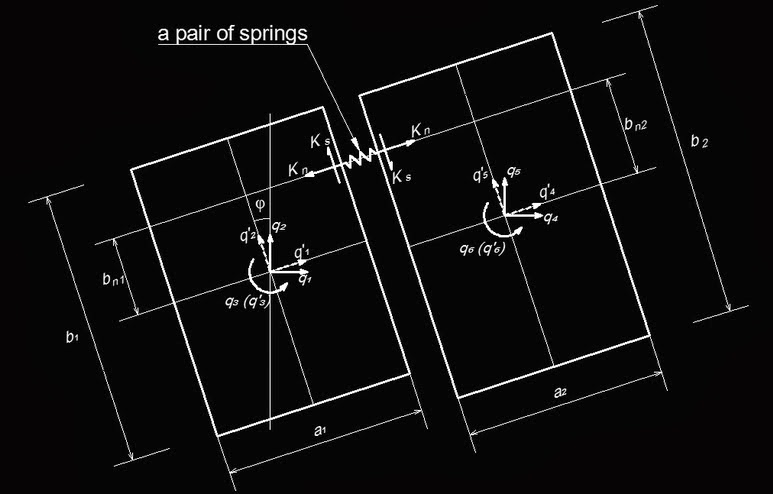
\includegraphics[width=0.8\textwidth]{../stiffness_matrix_elements.jpg}
\caption{Two elements with normal and shear spring connection [\cite{Blog_python_AEM}]}
\label{fig:stiffness_matrix_elements}
\end{figure}


The translation matrix are:
\begin{equation}
L = 
\begin{bmatrix}
cos(\varphi) & sin (\varphi) & 0 & 0 & 0 & 0 \\
- sin (\varphi) & cos (\varphi) & 0 & 0 & 0 & 0 \\
0 & 0 & 1 & 0 & 0 & 0 \\
0 & 0 & 0 & cos (\alpha) & sin (\alpha) & 0 \\
0 & 0 & 0 & - sin (\alpha) & cos (\alpha) & 0 \\
0 & 0 & 0 & 0 & 0 & 1 \\
\end{bmatrix}
\end{equation}

The stiffness matrix can then be calculated by the above mentioned method of a unit displacement in each degree of freedom and calculating the forces at the centroid of the elements. 
This is the stiffness matrix for the local co-ordinate system:
\begin{equation}
K^{te} = 
\begin{bmatrix}
K_n & 0 & -K_n b_{n1} & -K_n & 0 & K_n b_{n2} \\

0 & K_s & K_s \frac{a_1}{2} & 0 & -K_s & K_s \frac{a_2}{2} \\

-K_n b_{n1} & K_s \frac{a_1}{2} & K_n (b_{n1})^2 + K_s (\frac{a_1}{2})^2 & K_n b_{n1} & -K_s \frac{a_1}{2} & -K_n (b_{n1} b_{n2}) + K_s (\frac{a_1}{2} \frac{a_2}{2}) \\

-K_n & 0 & K_n b_{n1} & K_n & 0 & -K_n b_{n2}  \\

0 & -K_s & -K_s \frac{a_1}{2}& 0 & K_s & -K_s \frac{a_2}{2} \\

K_n b_{n2} & K_s \frac{a_2}{2} & -K_n (b_{n1} b_{n2}) + K_s (\frac{a_1}{2} \frac{a_2}{2}) & -K_n b_{n2} & -K_s \frac{a_2}{2} & K_n (b_{n2})^2 + K_s (\frac{a_2}{2})^2 \\
\end{bmatrix}
\label{eq:Kte matrix}
\end{equation}

Now the stiffness matrix can be calculated as 
\begin{equation}
K^e = L^T K^{te} L
\end{equation}

End of section extracted from [\cite{Blog_python_AEM}].

Note that this stiffness matrix computed above is only for one spring.  To calculate the stiffness matrix for more springs the same procedure is followed and then the matrices are added together to form the stiffness matrix.  Note that logic then dictates that the stiffness matrix size is not dependant on the amount of springs but rather the amount of elements.  The final stiffness matrix is thus an average for the element according to the stress situation around the particular element.  In this case pure rigid body motion of each element is considered and thus the stress is proportional to the displacement between the two ends of the springs.  The strain is firstly calculated using:

\begin{eqnarray}
\epsilon_x = \frac{d_x}{a} \\
\epsilon_y = \frac{d_y}{a} 
\end{eqnarray}

For each spring either the x displacement or the y displacement can be calculated.  Note that $d_x$ and $d_y$ are relative displacements of spring ends.  The stresses is then simply calculated as

\begin{eqnarray}
\sigma_x = E \epsilon_x \label{eq:stress_x} \\
\sigma_y = E \epsilon_y \label{eq:stress_y}
\end{eqnarray}


Note how for purely translational purposes a single spring would be adequate as the stiffness is calculated using the area represented by the spring and summing a bunch of springs together for a purely translational load leads to the same result as using one spring for the entire area.  However using more springs leads to a greater accuracy for rotational loading to prove this the theoretical stiffness using only normal springs were calculated and then compared to the stiffness computed using a finite amount of normal springs. 
The process can easily be proved by writing out all the equations, I summarized the results below:

Referring to Figure \ref{fig:rotational_accuracy_AEM} the following should be noted:
\begin{itemize}
	\item The elements are square thus $a$ as used in Equations \ref{eq:Normal_spring} and \ref{eq:Shear_spring} are the same as b in Figure \ref{fig:rotational_accuracy_AEM}
	\item The number of connecting springs are $2n$ thus the minimum number of springs are 2
	\item The rotational stiffness contribution of the normal springs are $K_r = K_n z^2$
\end{itemize}

Theoretically thus the stiffness for rotation are:

\begin{eqnarray}
K_r = \int_{y = -\frac{b}{2}}^{y = \frac{b}{2}} \frac{ET}{b} z^2 dz \\
K_r = \frac{ETb^2}{12} 
\label{eq:infinite_rot_stiff}
\end{eqnarray}

\begin{figure}[H]
\centering
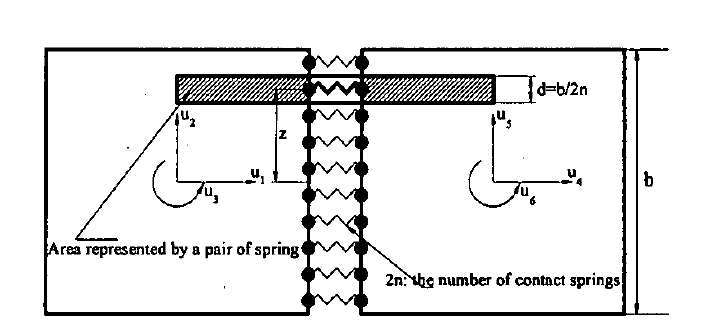
\includegraphics[width=0.5\textwidth]{../rotational_accuracy_AEM.png}
\caption{Effects of number of springs on rotational stiffness [\cite{First_AEM}]}
\label{fig:rotational_accuracy_AEM}
\end{figure}

The stiffness calculated from $2n$ springs are then:

\begin{equation}
K_r =  \frac{ETb^2}{4n^3} \Sigma^{n}_{i=1}(i - 0.5)^2
\label{eq:finite_rot_stiff}
\end{equation}

The resulting comparison shows that more springs result in smaller errors when comparing equations \ref{eq:infinite_rot_stiff} and \ref{eq:finite_rot_stiff}.  The same error difference was obtained in my own comparison as in the paper namely:

\begin{itemize}
\item $25 \%$ for 2 springs
\item $2.8 \%$ for 6 springs
\item $1.0 \%$ for 10 springs
\item $0.3 \%$ for 20 springs
\end{itemize}

The final equation to solve, as with FEM, is:

\begin{equation}
K_G U=F
\end{equation}

Here $K_G$ is the global stiffness matrix, $U$ the displacement vector and $F$ the applied forces. 
The same method is used for both load and displacement control cases.  For load cases the vector F is already known and we simply solve for U.  "In displacement control cases, the load is applied by unit virtual displacement for one or more degrees of freedom." [\cite{First_AEM}] \textcolor{blue}{I am unsure how exactly to implement this}
 
Note that the matrix in Equation \ref{eq:Kte matrix} is symmetrical.  Thus after computing the global stiffness matrix a vector can be created for half the matrix containing only the non zero elements, thus saving memory and computing time.  The layout of the program is shown in the Figure \ref{fig:AEM_flow_chart}.  Note how the stiffness matrix is recomputed for each increment. 

\begin{figure}[H]
\centering
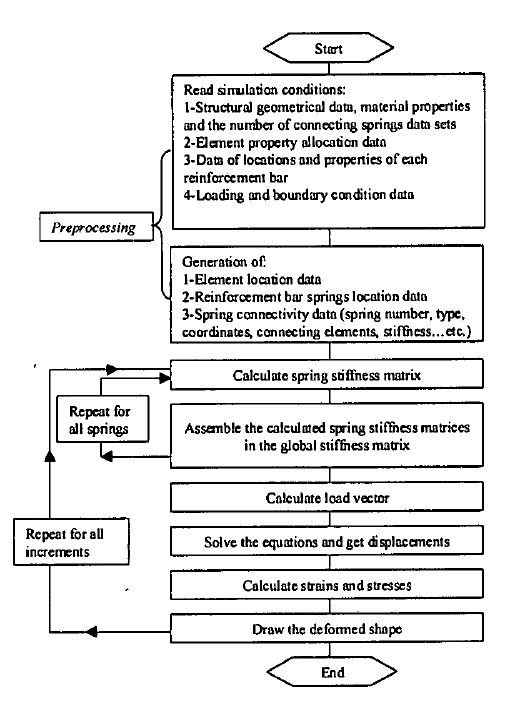
\includegraphics[width=0.5\textwidth]{../AEM_flow_chart.png}
\caption{Flow chart of an elastic loading condition AEM program [\cite{First_AEM}]}
\label{fig:AEM_flow_chart}
\end{figure}

The number of elements and their influence was studied in [\cite{First_AEM}] included was also the amount of springs used between elements.  Final conclusions were that more elements with lower number of springs lead to more accuracy and less CPU time than high number of springs between elements.  To improve the accuracy in the case of elastic modelling it was advised to use higher number of elements with less springs for example 10 springs rather than 20.  It was found that the same accuracy was obtained for 10 springs as for 20 springs but with half the CPU time.  In conclusion it was found that larger elements are sufficient for cases where normal stresses are the most important but smaller and more elements are needed to accurately predict the shear stresses. 

\subsubsection{Poisson Effect}

According to [\cite{First_AEM}] there are two ways to model for the Poisson effect.  \textcolor{blue}{I think these might be used to model the thermal expansion as well if adapted}


\paragraph{First Method} The first method introduces two additional degrees of freedom to the 2D model.  Thus each element now has two additional degrees of freedom and results in a total of 5 degrees of freedom namely, x and y displacement, rotational and the expansion in the y and x direction.  This however increases CPU time by approximately 2.78.  The other additional problem is that DOF's now have a coupling effect making it harder to calculate the stresses and strains in the elements. 

\paragraph{Second Method}  The second method involves still using only three degrees of freedom, but takes advantage of the assembly of the elements which is deformable.  The stiffness matrix of each element is correlated by those of adjacent elements.  This is the preferred method according to [\cite{First_AEM}] because it avoids the problems mentioned for the previous method.  \textcolor{blue}{Both should be investigated as possible solutions for the temperature expansion though}

Firstly a factor needs to be introduced which will govern whether forces due to Poisson ratio expansion should be included in the stiffness matrix or not.  This factor is calculated according to numbering of elements and of element edges.  This is illustrated in Figure \ref{fig:Poisson_element_numbering_AEM}.

\begin{figure}[H]
\centering
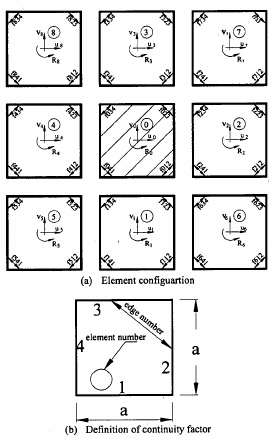
\includegraphics[width=0.4\textwidth]{../Poisson_element_numbering_AEM.png}
\caption{Element and element edge numbering used in Poisson effect inclusion [\cite{First_AEM}]}
\label{fig:Poisson_element_numbering_AEM}
\end{figure}

The factor is then calculated using equation \ref{eq:element_continuity}.  In this case the element is divided into four sections with $i$ indicating element number and $j$ and $k$ the edge numbers.  If there is no element connected (springs need to be active) to element $i$ at edge $j$ then $fij=0$.  If there is a connecting element then $fij=1$.  

\begin{equation}
fijk = fij \times fik
\label{eq:element_continuity}
\end{equation}

Remember that for each spring a stiffness matrix is developed and then all these are summed together to form the stiffness matrix for the element.  Now additional terms need to be added, these are calculated by assuming a corresponding displacement in the direction of the studied DOF and then calculating the response at the centre of the element.  Thus these terms are added to the already assembled stiffness matrix of each element. 

\begin{figure}[H]
\centering
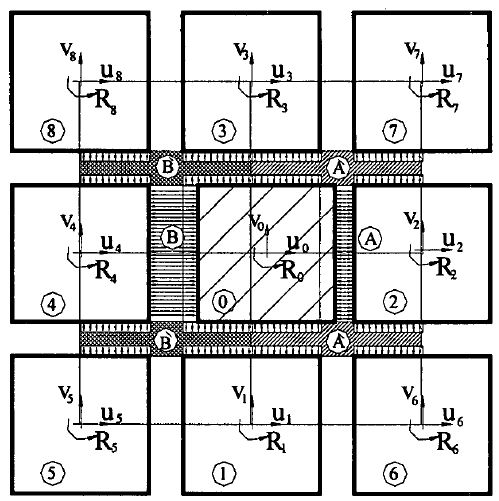
\includegraphics[width=0.4\textwidth]{../Poisson_effect_element_grid_AEM.png}
\caption{Horizontal displacement of element 0 with Poisson effect taken into account [\cite{First_AEM}]}
\label{fig:Poisson_effect_element_grid_AEM}
\end{figure}

From Figure \ref{fig:Poisson_effect_element_grid_AEM} it can be seen that due to horizontal displacement of element 0 region A is compressed and region B experiences tension.  This means that a secondary stress is induced in areas A` and B` due to lateral displacement which is a function of the Poisson ratio.  Note that if the lateral displacement is not prevented no additional stiffness matrix terms will have to be included.  This is why the factor for continuity was introduced in equation \ref{eq:element_continuity}. 

In the case of element rotation, the secondary stresses induced are assumed to be evenly distributed across element faces. From [\cite{First_AEM}] the additions to the global stiffness matrix, for unit displacements in all DOF for element one, are recorded in Figure \ref{fig:Poisson_additions_stifmat_AEM}.  As this is a system with 9 elements each having 3 DOF the final matrix size will be $27 \times 27$.  Those shown in Figure \ref{fig:Poisson_additions_stifmat_AEM} are the first three rows. 

\begin{figure}[H]
\centering
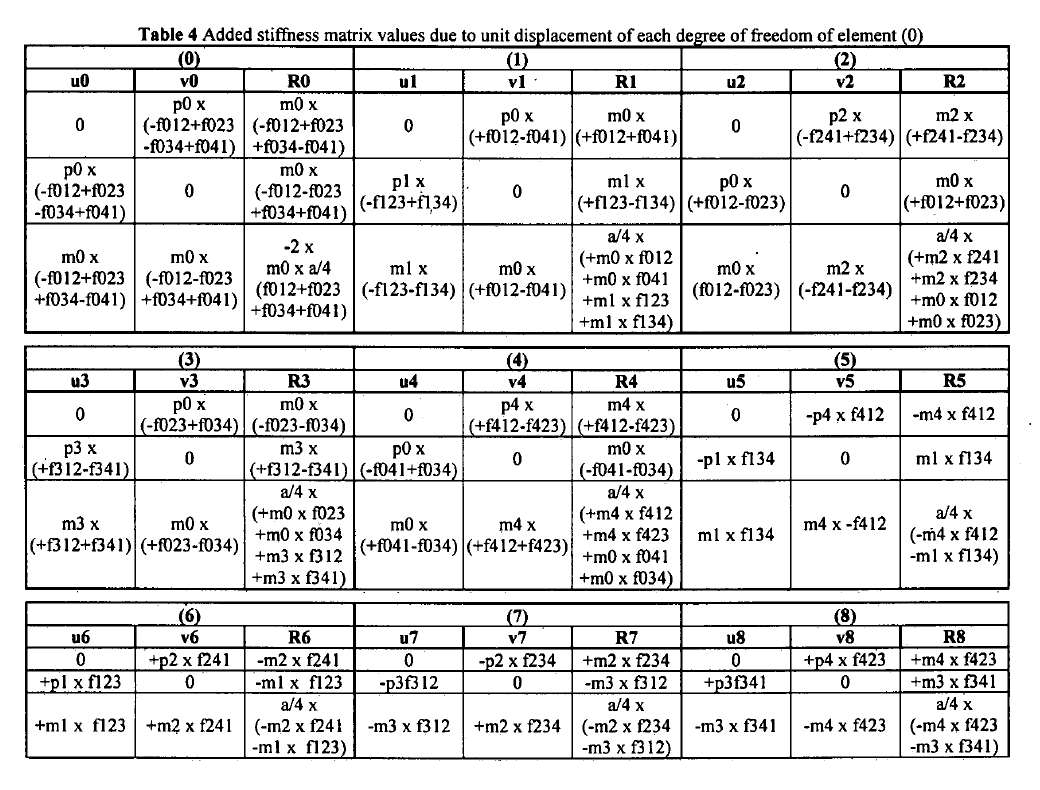
\includegraphics[width=0.8\textwidth]{../Poisson_additions_stifmat_AEM.png}
\caption{Values to add to stiffness matrix for unit displacement in all DOF for element one in Figure \ref{fig:Poisson_effect_element_grid_AEM} [\cite{First_AEM}]}
\label{fig:Poisson_additions_stifmat_AEM}
\end{figure}

The force and moments imposed are

\begin{eqnarray}
pi = \frac{\nu E_i t_i}{4(1-\nu^2)} \\
mi = \frac{\nu E_i t_i}{4(1-\nu^2)} \times \frac{a}{4}
\end{eqnarray}

$\nu$ is the Poisson ratio with E and t being the Young's Modulus and the element thickness respectively.  $i$ indicates the element number.  Note the role he continuity factor plays in the assembly of the matrix, if a neighbouring element does not exist or if contact springs aren't in place due to cracking the effect is not taken into account.  Also notice that only the forces and moments due to the normal springs are adjusted. 

To calculate the stresses some alterations need to be made to equations \ref{eq:stress_x} and \ref{eq:stress_y}.  Firstly an average strain need to be calculated for each element namely $\epsilon_{xa}$ and $\epsilon_{ya}$ and then the new stress equations are:

\begin{eqnarray}
\sigma_x = E \times \frac{\epsilon_x + \nu \epsilon_{ya}}{1-\nu^2} \\
\sigma_y = E \times \frac{\epsilon_y + \nu \epsilon_{xa}}{1-\nu^2}
\end{eqnarray}

Notice that when the Poisson ratio is ignored, $\nu=0$ then we obtain equations \ref{eq:stress_x} and \ref{eq:stress_y} again. 






 
